\documentclass[UTF8,a4paper,11pt,fontset=fandol]{ctexart}
\usepackage[margin=23mm]{geometry}
\usepackage{amsmath,amssymb,booktabs,longtable,graphicx,float,fancyhdr,xcolor,needspace}
\usepackage{xurl}
\usepackage[unicode,colorlinks=true,linkcolor=black,urlcolor=blue]{hyperref}
\definecolor{accent}{HTML}{155574}
\pagestyle{fancy}
\fancyhf{}
\fancyhead[L]{\small 数学建模训练论文}
\fancyhead[R]{\small 待人工审阅}
\fancyfoot[C]{\thepage}
\setlength{\headheight}{15pt}
\setlength{\parskip}{0.35em}
\setlength{\emergencystretch}{3em}
\title{\bfseries 训练工坊的整数生产配置与资源情景分析}
\author{}
\date{}
\begin{document}
\maketitle
\vspace{-2.4em}
\begin{center}\small\color{accent}训练草稿：计算已核验，建模解释、引用及赛事格式仍需队员审阅\end{center}
\begin{abstract}
针对训练工坊的生产配置任务，建立满足最低与最高产量要求的整数线性规划模型。原始机时容量为 19，材料容量为 21。实际求解利润为 122.00，可行贪心基线利润为 103.00，相对变化为 18.45\%。通过约束复算和整数域枚举核验主方案，并比较资源同步变化的情景。结论限于题目声明的人工构造数据。
\end{abstract}
\noindent\textbf{关键词：}整数生产配置；容量约束；枚举核验；情景分析

\section{问题分析与数据来源}
用户提供的生产配置训练任务及 products.csv，原题明确数据为人工构造；不代表实际企业测量。
\begin{description}

\item[Q1] 按附件最低与最高产量约束给出利润最大的整数生产方案，并与可行基线比较。

\item[Q2] 比较资源容量同步收缩或扩张时的目标变化。

\end{description}

\section{模型假设与符号}
\begin{enumerate}

\item 决策期内各产品的单位利润与单位资源消耗固定。

\item 产品按整件生产，最低与最高产量均按原始附件严格约束。

\item 情景分析只同步改变资源容量，其余参数保持不变。

\end{enumerate}
\begin{longtable}{p{.16\textwidth}p{.46\textwidth}p{.20\textwidth}}
\toprule 符号 & 含义 & 单位 \\ \midrule

x\_1 & 训练品A & 件 \\

x\_2 & 训练品B & 件 \\

x\_3 & 训练品C & 件 \\

\bottomrule
\end{longtable}

\section{模型建立与求解方法}
决策变量是整数，目标和资源约束均线性；使用 MILP 并与线性松弛上界比较。

\begin{equation}
\max\; z=\sum_{j=1}^{n}p_jx_j
\end{equation}

\begin{equation}
\sum_{j=1}^{n}a_{ij}x_j\leq b_i\quad(i=1,\ldots,m)
\end{equation}

\begin{equation}
l_j\leq x_j\leq u_j,\quad x_j\in\mathbb{Z}_{\geq0}
\end{equation}

\noindent\textbf{基线方案：}从最低产量出发，按单位归一化资源利润贪心增量配置；若最低产量不可行则报告不可行。


\section{主方案与约束解释}
依据附件的利润、资源消耗和产量边界建立模型。原题要求产品按整件生产，且训练品A对应的最低生产数量必须保留。使用 SciPy 的混合整数规划求解接口[scipy\_milp]，得到目标值 122.00；线性松弛上界为 123.67。可行贪心基线目标值为 103.00，相对变化为 18.45\%。各产品的具体配置数量见结果表。求解状态与数值核验共同作为最优性表述依据。

\section{容量情景与局限}
对两类资源容量实施同步比例扰动，逐个重新求解并保留状态，具体数值见情景表。由于整数产量约束，增加容量的效益可能存在台阶。本次同步扰动不等价于每类资源的独立边际价值分析；实际业务解释还需要核验利润和资源消耗的稳定性。


\section{计算结果与图表}
所有数值均读取同一次实验记录；表中的不可用项保留其原始状态。

\Needspace{7\baselineskip}
\subsection*{生产配置方案}
{\small
\begin{longtable}{lll}
\toprule
产品 & 数量 & 利润 \\ 
\midrule\endhead

训练品A & 6 & 66 \\ 

训练品B & 7 & 56 \\ 

训练品C & 0 & 0 \\ 

\bottomrule
\end{longtable}}

\Needspace{7\baselineskip}
\subsection*{资源容量情景}
{\small
\begin{longtable}{lll}
\toprule
容量倍率 & 求解状态 & 目标值 \\ 
\midrule\endhead

0.9 & 最优 & 107 \\ 

1 & 最优 & 122 \\ 

1.1 & 最优 & 130 \\ 

\bottomrule
\end{longtable}}


\begin{figure}[H]
\centering
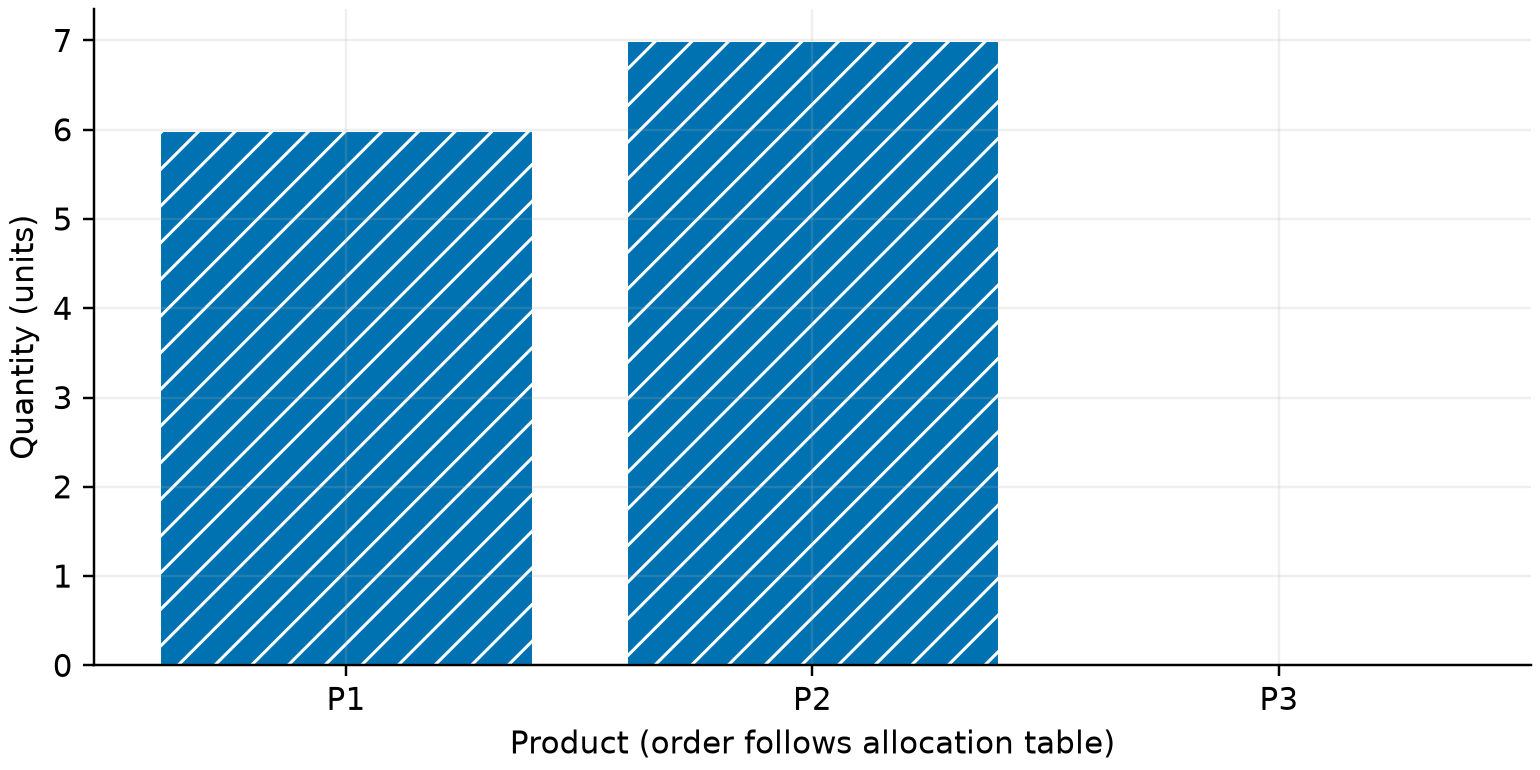
\includegraphics[width=.91\textwidth]{../figures/allocation.png}
\caption{各产品的整数配置数量；产品顺序与配置表一致。}
\end{figure}

\begin{figure}[H]
\centering
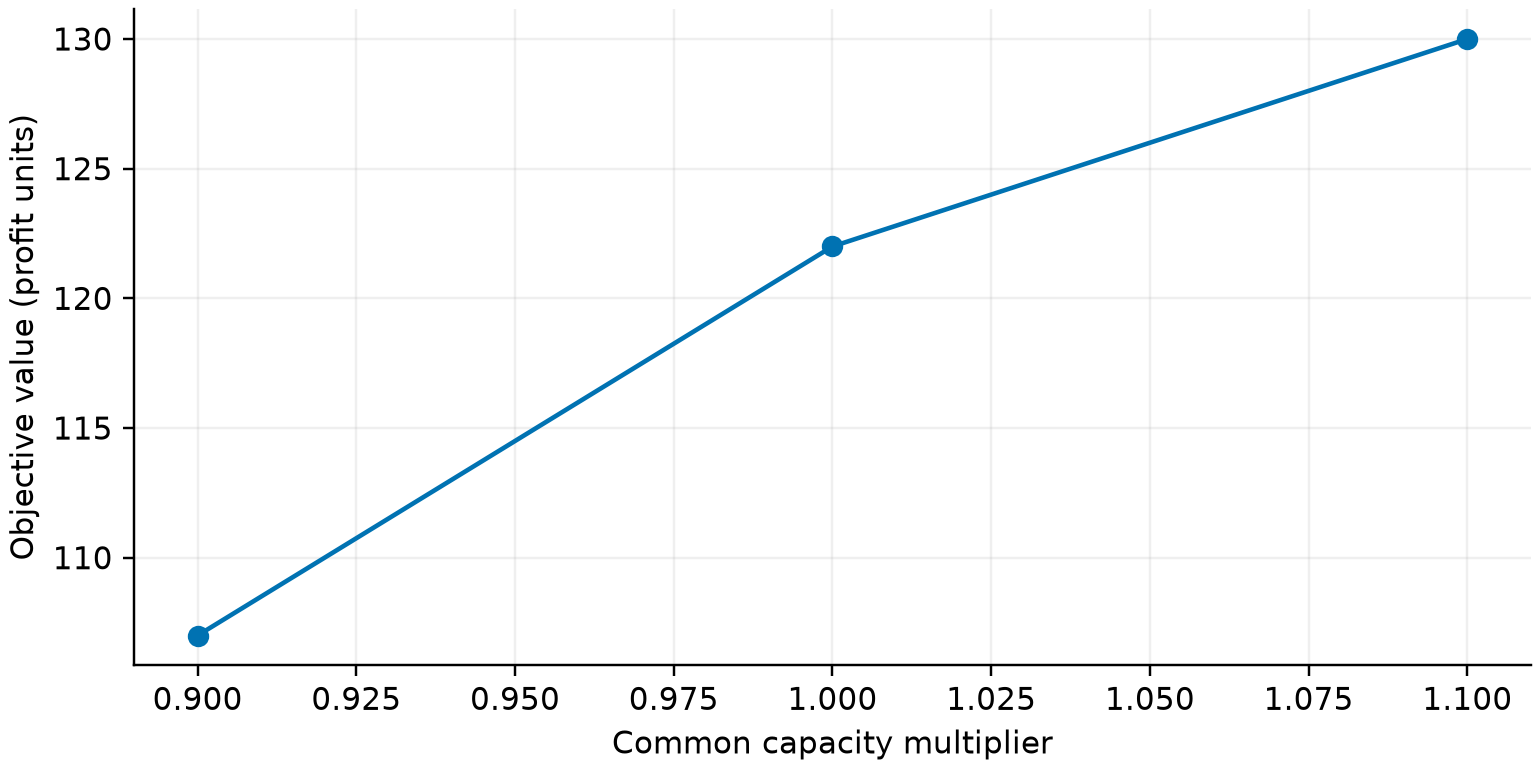
\includegraphics[width=.91\textwidth]{../figures/sensitivity.png}
\caption{全部资源容量同步变化时的目标值；不可行情景不绘制数值。}
\end{figure}


\section{检验、局限与改进方向}
本次自动核验覆盖了已编码的数值条件。自动核验通过不等价于题意解释已经充分，队员仍需对照原题审阅假设与结论。
\begin{itemize}

\item 利润与资源消耗视为常数，未包含价格反馈。

\item 情景扰动属于局部分析，不代表随机鲁棒最优。

\end{itemize}

\section*{参考来源}

\begin{description}

\item[scipy\_milp] SciPy 官方文档：混合整数线性规划 milp. \url{https://docs.scipy.org/doc/scipy/reference/generated/scipy.optimize.milp.html}. 核验状态：opened\_by\_agent.

\end{description}

\section*{复现与 AI 使用说明}
数据来源、程序版本和输入摘要见工作区中的 provenance.json；运行命令见复现说明。
本案例使用已声明的训练数据，结论仅用于演示建模过程。
实际 AI 工具使用、人工修改及核验记录保存在 ai\_usage.jsonl 中，由队员据实补充后按赛事要求整理。
\end{document}